\section[Measuring Beliefs II]{Measuring Beliefs II \iftoggle{showdates}{\small{\textit{2014-05-09}}}{}}

\subsection{Probabilities of Continuous Random Variables}
How tall is Frank Jäkel? 1.80m, 1.70m, 1.68m, 1.69m, or even 1.7034241m?

Not only are there problems with real numbers like 1.7034241, but also with the question the Bayesian view inevitably asks: ``What do you think is the probability for that size?''

One sees: continuous random variables are difficult. There is an infinite uncountable range of numbers and one shall assign probabilities for them. This leads straight to the question: ``What's the probability of a real number?''

In the following section this problem gets tackled in three ways.

\subsubsection[Probability Density Function (PDF)]{Solution 1: Histograms (Probability Density Function, PDF)}
The first and naive way is to discretize the sample space $\mathbb{R}$ into bins and assign probabilities to those bins.

\begin{center}
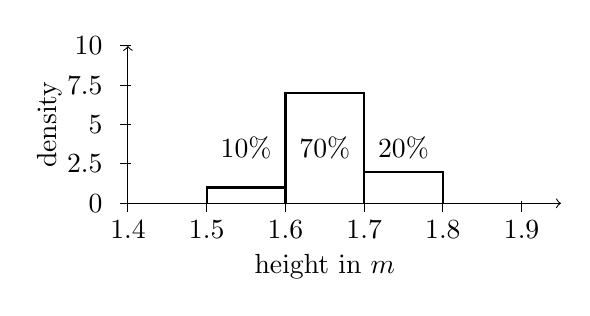
\begin{tikzpicture}

  % horizontal axis
  \draw[->] (0, 0) -- (5.5, 0);
  % ticks horizontal
  \foreach \x in {0,...,5}
    \draw (\x,1pt) -- (\x,-3pt);
  % labels horizontal
  \draw	(0,-0.1) node[anchor=north] {1.4}
		    (1,-0.1) node[anchor=north] {1.5}
		    (2,-0.1) node[anchor=north] {1.6}
		    (3,-0.1) node[anchor=north] {1.7}
		    (4,-0.1) node[anchor=north] {1.8}
		    (5,-0.1) node[anchor=north] {1.9}
        ;
  % axis label
  \draw (2.5,-0.8) node {height in $m$};
  
  % vertical axis
  \draw[->] (0, 0) -- (0, 2);
  % ticks vertical
  \foreach \y in {0,0.5,1,1.5,2}
    \draw (1pt, \y) -- (-3pt, \y);
  % labels vertical
  \draw (-0.2,0.0) node[anchor=east]  {0}
        (-0.2,0.5) node[anchor=east]  {2.5}
        (-0.2,1.0) node[anchor=east]  {5}
        (-0.2,1.5) node[anchor=east]  {7.5}
        (-0.2,2.0) node[anchor=east] {10}
        ;
  % axis label
  \draw (-1,1) node[rotate=90] {density};
  
  % first box
  \draw[thick] (1, 0) -- (1, 0.2) -- (2, 0.2) -- (2, 0);
  % second box
  \draw[thick] (2, 0) -- (2, 1.4) -- (3, 1.4) -- (3, 0);
  % third box
  \draw[thick] (3, 0) -- (3, 0.4) -- (4, 0.4) -- (4, 0);
  
  % box labels
  \draw (1.5,0.7) node{$10 \%$};
  \draw (2.5,0.7) node{$70 \%$};
  \draw (3.5,0.7) node{$20 \%$};
  
\end{tikzpicture}
\end{center}

Note that \textbf{the area describes the probability}. For the second box, we would assign a y-value of 7, such that the width (0.1) times the height equals the probability ($0.1\cdot 7 = 0.7$).

\textit{From here on it's just notes for the rest of this section, working on it!}

Histogram! -> Limit of the histogram: Probability density function (PDF)
Make discrete space: 150-160, 160-170, etc.
Assign probabilities to those bins.
Change resolution (150-155, 155-160), reassign/reorder 

this is the density (and it's = 1 (area/integral))

two weird extreme cases:
- reassigning/reordering causes high densities
- equally distributed density causes probability of 0 for each exact number
   - however, you can calculate the probability for intervals with the integral
   -> you only want to bet on intervals

\subsubsection[Cumulative Density Function (CDF)]{Solution 2: Cumulative Density Function, CDF}
CDF is the integral of the PDF
 % rest see paper notes

\subsubsection{Solution 3: Parametric Distribution}
We use the Gaussian distribution

\begin{align*}
p(X=x) &= \frac{1}{2\pi\sigma^2}e^{-\frac{1}{2}\left(\frac{\mu-x}{\sigma}\right)^2} = \phi(x;\mu,\sigma) = \phi\left(\frac{\mu-x}{\sigma};0,1\right) \\
\frac{\mu-x}{\sigma}&=z \\
P(X \leq t) &= \int\limits_{-\infty}^{t}{p(X=x)} dx = \Phi(t;\mu,\sigma) \\
\mbox{probability of the standard deviation: } \\
P(\mu\sigma \leq X \leq \mu + \sigma) &= \Phi(\mu+\sigma;\mu,\sigma) - \Phi(\mu-\sigma;\mu,\sigma) \approx 68\%
\end{align*}

\begin{itemize}
	\item $\mu \pm \sigma \approx 68\%$
	\item $\mu \pm 2\sigma \approx 95\%$
	\item $\mu \pm 3\sigma \approx 99\%$
\end{itemize}

\subsection{Proper Scoring Rules}
Multiple choice test: better to say: ``How is your belief that this is right''

Example: EU pop > US pop? X = 1 if true, X = 0 if false

aim: high gain if true and high q, no gain if high q but false etc.

q is what you say your belief is 
\begin{align*}
L(X,q) &= (X-q)^2 \\
       &= X^2-2qX+q^2 \mbox{ note: $X^2 = X$, since only 1 or 2} \\
       &= X(1-2q)+q^2
\end{align*}

You lie: Your true belief is p, but you say q.

For best performance on test minimize expected loss $E(L(X,q)) = p(1-2q)+q^2$

p is ``a bet on $p\cdot num$ of questions are true'', so that's why the expected loss is like this

Minimize E: $1^{st}$ derivative:
\begin{align*}
E(L(X,q)) &= p(1-2q)+q^2 \\
\frac{\partial E}{\partial q}E(L(X,q)) &= -2p + 2q \\
\Leftrightarrow p = q
\end{align*}




